\documentclass[preprint]{aastex63}
\usepackage{amsmath}
\usepackage{url}
\usepackage{hyperref}
\usepackage[utf8]{inputenc}
\setlength{\parindent}{3ex}
\usepackage{caption}
\usepackage{subcaption}

\usepackage{natbib}

\begin{document}
\title{CTA-200H Computing Course Project: The Microlensing Phenomenon}
\author{Xiaoyi Ma}




\section{Single-lens Microlensing \& Parallax Effect}
\medskip
\subsection{Paczynski Curve Model}

The Pacynsiki curve is a smooth and symmetric light curve that describe the magnification of the source (with angle $\beta$ respect to lens) to the image (with angle $\theta$ respect to lens) with respect to time. The curve can be described as following equation 1, where A is the total magnification that is the inverse of the determinant of the Jacobian matrix for the lens equation \cite{2012ARA&A..50..411G}.

\begin{equation}
    A(u(t)) = \frac{u^2+2}{u\sqrt{u^2+4}}
\end{equation}

In the above equation, $u$ is defined as $\beta/\theta_E$. Since the source, lens and observer are in relative motion, $u$ is dependent on time that can be described as following equation 2 \cite{2012ARA&A..50..411G}.

\begin{equation}
    u=[(\frac{t-t_0}{t_E})^2+u_0^2]^{1/2}
\end{equation}

In the above equation, t is the time for the lensing event. There are three parameters in equation 2. $u_0$ is the impact parameter of the lensing event that indicated the minimum projected separation between the source and lens (closest alignment) \cite{Poleski_2019}. $t_0$ is the time when $u=u_0$, where the magnification is at its maximum. $t_E$ is time cross Einstein ring, which is defined as Einstein ring radius over the lens-source relative proper motion $\theta_E/\mu_{rel}$ \cite{2012ARA&A..50..411G}. Therefore, according to two equations above, the three parameters $t_0$,$u_0$,$t_E$ define the magnification that is the Pacynsiki curve.

\bigskip
\subsection{Graph for Paczynski Curve Model Without Parallax}

The Paczynski light curve for $t_0=2459031.5JD$, $t_ E=100$ days and different impact parameters $u_0=(0.1,\,0.3,\,1.0)$ for point-Source is plotted in Figure 1 via \texttt{MulensModel.magnificationcurve} module \cite{Poleski_2019} with a scale 2.5$log_{10}(A)$ and time range of [$-2t_{\rm E}$, $2t_{\rm E}$].  As we can see from the graph, the light curve reaches its peak at $t_0$. As $u_0$ getting close to 1.0 where $\beta$ getting close to $\theta_E$, the amplitude of magnification peak gets greater.\clearpage

\begin{figure}[h]
\centering
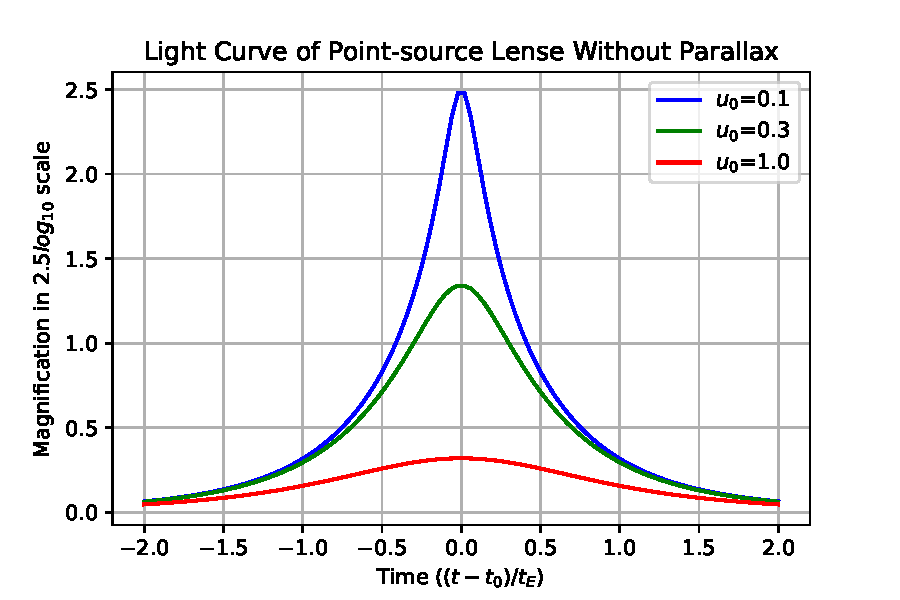
\includegraphics[width=.5\textwidth]{1.2.png}
\caption{Light Curve of Point-Source Lens Without Parallax}
\label{fig 1}
\end{figure}

\bigskip
\subsection{Graph for Paczynski Curve Model With Parallax}
The graph of light curve of the lens event with $u_0=0.3$ is plotted in Figure 2a, where the dash line represents the event without parallax, and the solid line represents the event with parallax parameter $(\pi_{\rm E,N},\,\pi_{\rm E,E})=(0,\,0.5)$ and $(0.5,\,0)$. As we can see from the graph, for the range near the peak, the light curve of three event coincide with each other. The difference between three curves gets greater away from the peak. For the graph the of the trajectory of the source (Figure 2b), the trajectory of the non-parallax case is a straight line, and the trajectory of the parallax cases is the same that is away from the straight trajectory due to Earth's orbital motion. The code for 1.2 and 1.3 is the file microlensing-1.py.

\begin{figure}[h]
\centering
\begin{subfigure}{.49\textwidth}
  \centering
  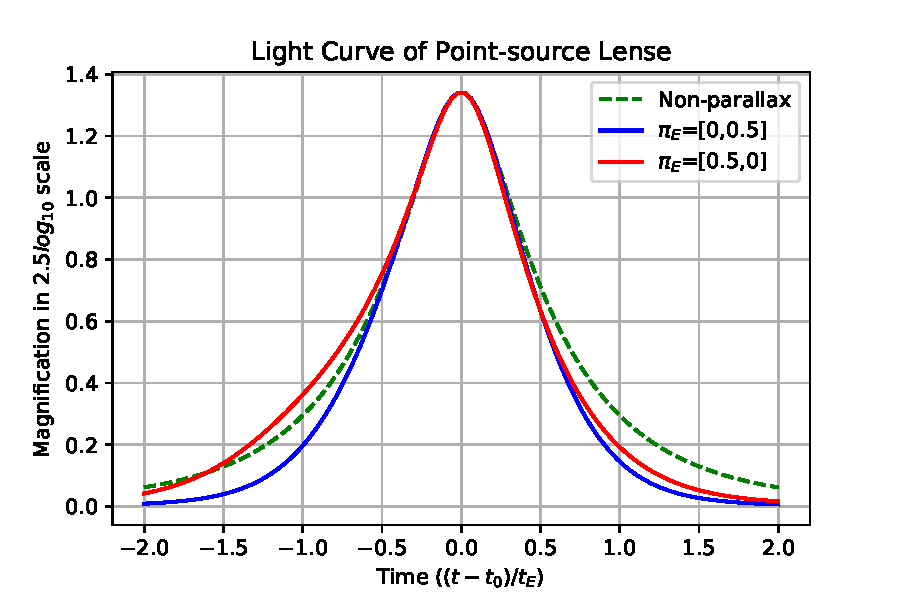
\includegraphics[width=\textwidth]{1.3.1.png}
  \caption{Light Curve}
\end{subfigure}
 \begin{subfigure}{.49\textwidth}
  \centering
  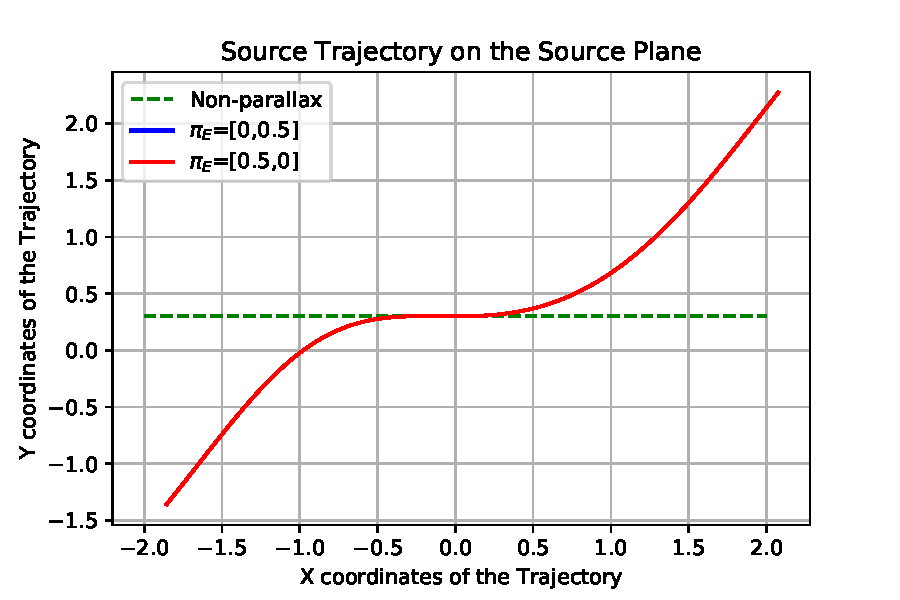
\includegraphics[width=\textwidth]{1.3.2.png}
  \caption{Trajectory of Source}
 \end{subfigure}
\caption{Light Curve and Trajectory for Lens Event With and Without Parallax}
\label{fig 2}
\end{figure}

\bigskip
\subsection{Signatures of Lensing Event}

$\pi_E$ and $t_E$ are both related to the Einstein angle that defined as following formula, which is proportional to $\sqrt{M_L}$.

\begin{equation}
    \theta_E = \sqrt{\frac{4GM_L}{D_{rel}c^2}}=713\mu as (\frac{M_L}{0.5M_\odot})^{1/2}(\frac{\pi_{rel}}{125 \mu as})^{1/2}
\end{equation}

$\pi_E$ is the parallax amplitude is equal to the ratio between the relative lens-source parallax parameter and the Einstein angle as $\pi/\theta_E$. Since $\pi=AU/D_{L}$ that is independent of the $M_L$,the parallax amplitude is proportional to the ${M_L}^{-1/2}$.In more details, it is  proportional to $\frac{1}{713\mu as} (\frac{M_L}{0.5M_\odot})^{-1/2}$\par
$t_E$ is time cross Einstein ring that is defined as $\theta_E/\mu_{rel}$ as stated. Since $\mu_{rel}$ is the the relative proper motion of the lens and source that is independent of the $M_L$,the parallax amplitude is proportional to the ${M_L}^{1/2}$. In more details, it is proportional to 24.8 (days)$(\frac{M_L}{0.5M_\odot})^{1/2}$ \cite{2012ARA&A..50..411G}.\par

For a white dwarf, its lens mass ($M_L$) is small than Chandrasekhar limit that is 1.44 $M_\odot$ \cite{Carroll2007}. By the above scaling relation, the boundary value of the $\pi_E$ and $t_E$ are:
\begin{align*}
    \pi_E&\propto\frac{1}{713(\mu as)} (\frac{M_L}{0.5M_\odot})^{-1/2}\\
    &=\frac{1}{713(\mu as)} (\frac{1.44M_\odot}{0.5M_\odot})^{-1/2}\\
    &=0.00083 (\mu as^{-1})
\end{align*}
\begin{align*}
    t_E&\propto24.8 (days)(\frac{M_L}{0.5M_\odot})^{1/2}\\
    &=24.8 (days)(\frac{1.44M_\odot}{0.5M_\odot})^{1/2}\\
    &=42.09 (days)
\end{align*}


Therefore, $\pi_E\gtrsim0.00083 (\mu as^{-1})$ and $t_E\lesssim 42.09 (days)$ corresponds to the white dwarf.

For a neutron star, its lens mass ($M_L$) is small than Tolman–Oppenheimer–Volkoff limit that is taken as approximate 2.4$\M_\odot$\cite{Gao_2016}. Similar as above process,the boundary value of the $\pi_E$ and $t_E$ are:

   
$$\pi_E\propto\frac{1}{713(\mu as)} (\frac{2.4M_\odot}{0.5M_\odot})^{-1/2}=0.00064 (\mu as^{-1})$$
$$t_E\propto24.8 (days)(\frac{2.4M_\odot}{0.5M_\odot})^{1/2}=54.33 (days)$$

Therefore, $0.00064\lesssim\pi_E \lesssim 0.00083 (\mu as^{-1})$ and $42.09\lesssim t_E \lesssim 54.33 (days)$ corresponds to the neutron star.

For a stellar-mass black hole, its lens mass ($M_L$) is greater than 3.0 $M_\odot$. Similar as above process,the boundary value of the $\pi_E$ and $t_E$ are:

$$\pi_E\propto\frac{1}{713(\mu as)} (\frac{3.0M_\odot}{0.5M_\odot})^{-1/2}=0.00057 (\mu as^{-1})$$
$$t_E\propto=24.8 (days)(\frac{3.0M_\odot}{0.5M_\odot})^{1/2}=60.75 (days)$$

Therefore, $\pi_E \lesssim 0.00057 (\mu as^{-1})$ and $t_E \gtrsim 60.75 (days)$ corresponds to the stellar blackhole.
\medskip
\section{Binary-lens Microlensing \& Orbital Motion}
\bigskip
\subsection{Caustics Curve}
The equation for binary lens is equation 4, where $\zeta$ is the position of the source, z is the position of the image and $z_1$,$z_2$ are the position of the lens. They are all complex number where the real value is the x coordinate, imagery value is the y coordinate in the plane and the center of mass for two lens is the origin. $\epsilon$ is ratio the mass of the individual lens and sum of two masses \cite{2012ARA&A..50..411G}.
\begin{equation}
    \zeta=z-\frac{\epsilon_1}{\Bar{z}-\Bar{z_1}}-\frac{\epsilon_2}{\Bar{z}-\Bar{z_2}}
\end{equation}
Since the critical curve corresponds to the position where detJ=0 for the lens equation, therefore we can solve the points on critical curve with following equation 5 for each value of $\phi$ in the range of [0,2$\pi$] \cite{2012ARA&A..50..411G}.\par
\begin{equation}
    \frac{\epsilon_1}{(\Bar{z}-\Bar{z_1})^2}+\frac{\epsilon_2}{(\Bar{z}-\Bar{z_2})^2}=e^{i\phi}
\end{equation}
In order to solve equation 5 with \texttt{numpy.roots}, we need to expand equation 5 to a polynomial.
$$\epsilon_1(\Bar{z}-\Bar{z_2})^2+\epsilon_2(\Bar{z}-\Bar{z_1})^2-e^{i\phi}(\Bar{z}-\Bar{z_2})^2(\Bar{z}-\Bar{z_1})^2=0$$
Since $q=M_2/M_1$, we can express $\epsilon_1$ as $1/(q+1)$ and $\epsilon_2$ as $q/(q+1)$. Since the origin of the coordinate system is located at the center of mass for the binary system, $M_2\Bar{z_2}$+$M_1\Bar{z_1}$=0. Therefore $\Bar{z_1}$ and $\Bar{z_2}$ can be expressed with $s=\mid z_1-z_2 \mid$ and $q$, with following calculation.
$$\Bar{z_1}=-q\Bar{z_2}=s+\Bar{z_2}$$
$$\Bar{z_2}=\frac{-s}{q+1}$$
$$\Bar{z_1}=\frac{sq}{q+1}$$

For given $s$ and $q$, we can solve the polynomial of equation 5 for $\Bar{z}$ with 100 values of $\phi$ in [0,2$\pi$]. Then, $\zeta$ can be solved by substituting the values of $\Bar{z}$ and $z$ into equation 4, which corresponds to all points in the caustics curve.\par
The shape of the caustics curve that found with above algorithm in python is the same as the curve found with \texttt{MulensModel.caustics} module. The code for 2.1 is in the file microlensing-2.py.\par


\bigskip
\subsection{Binary Light Curve and Trajectory}
With timescale $t_{\rm E}=100$ days, impact parameter $u_0=0.1$, binary axis angle $\alpha=0$,the light curve of the binary lens is determined with \texttt{MulensModel.binarylens} module and \texttt{VBBL} method. The input source positions are determined with the \texttt{MulensModel.trajectory} module. The data for caustics curve is found with \texttt{MulensModel.caustics} module.\par
For part a, $\rho=10^{-3}$, $s=1.2$ and $q=(0.01,\,0.1,\,1)$, the light curve is shown in Figure 3a, caustics wave and trajectory of the source is the same for all $q$ that is a straight line are shown in Figure 3b. As the $q$ gets larger, the area enclosed by the caustics curve is larger.\par
For part b, $\rho=10^{-3}$, $q=0.1$ and $s=(0.8,\,1.0,\,1.2)$, the light curve is shown in Figure 3c, caustics wave and trajectory of the source that is a straight line are shown in Figure 3d. As the $s$ gets greater, the right side of caustic curve moves a lot toward the positive x direction and the left side moves a little toward the negative x direction. The y coordinate of caustics wave get closer to $x=0$ as the $s$ gets larger.\par
For part c, $q=0.1$, $s=1.2$ and $\rho=(10^{-3},\,10^{-2},\,10^{-1})$, the light curve is shown in Figure 3e, caustics wave and trajectory of the source that is a straight line are shown in Figure 3f. The variation in $\rho$ does not change the shape of the caustics curve. The code for 2.2 is in the file microlensing-3.py.\par

\bigskip
\begin{figure}[h]
\centering
\begin{subfigure}{.49\textwidth}
  \centering
  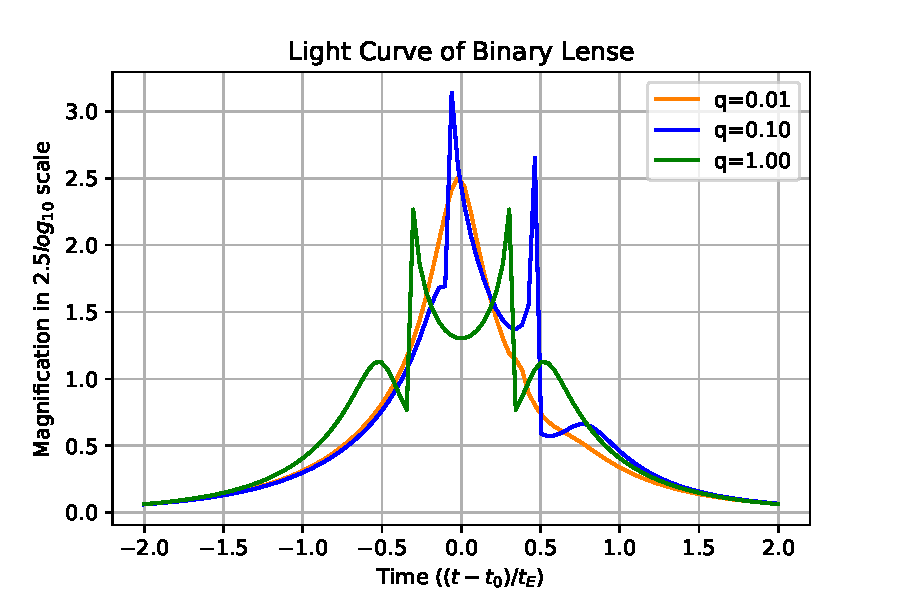
\includegraphics[width=\textwidth]{2_2a_l.png}
  \caption{Light Curve with Different $q$}
\end{subfigure}%
\begin{subfigure}{.49\textwidth}
  \centering
  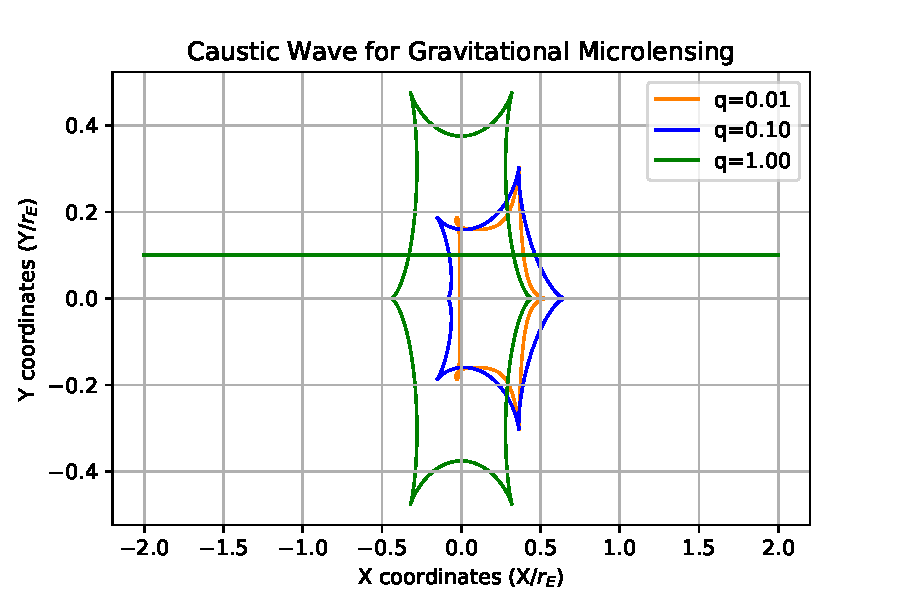
\includegraphics[width=\textwidth]{2_2a_c.png}
  \caption{Caustics Curve and Source Trajectory with Different $q$}
 \end{subfigure}
 \begin{subfigure}{.49\textwidth}
  \centering
  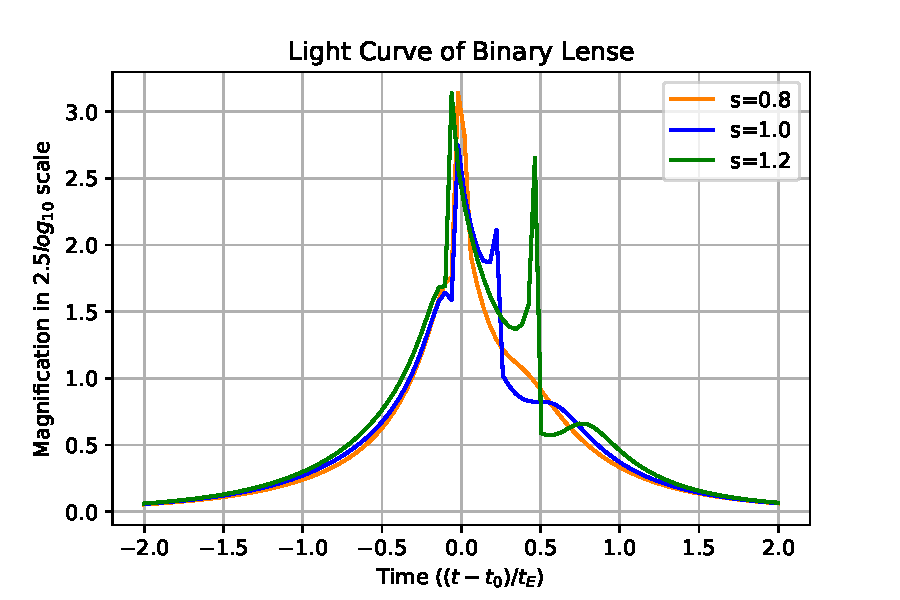
\includegraphics[width=\textwidth]{2_2b_l.png}
  \caption{Light Curve with Different $s$}
 \end{subfigure}
 \begin{subfigure}{.49\textwidth}
  \centering
  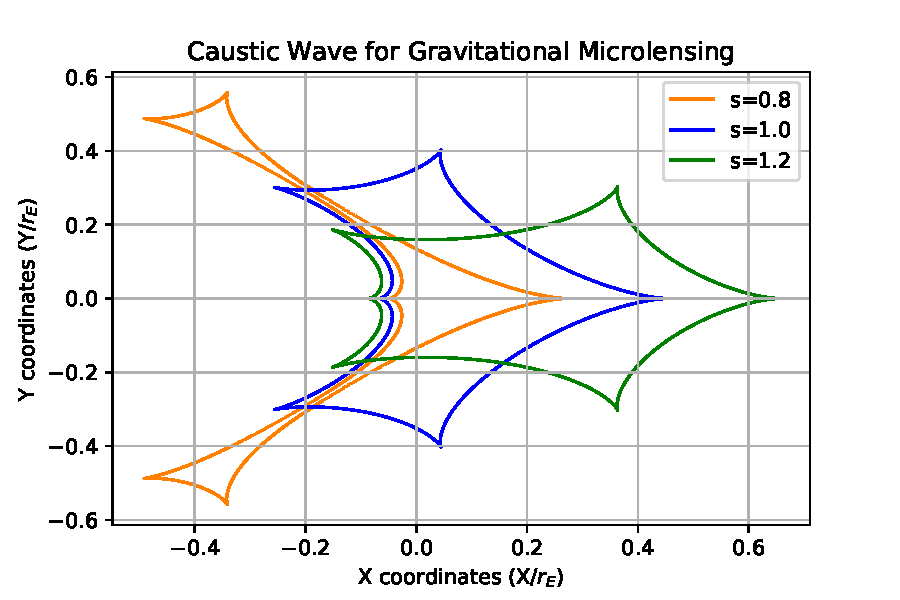
\includegraphics[width=\textwidth]{2_2b_c.png}
  \caption{Caustics Curve with Different $s$ }
 \end{subfigure}
\end{figure}%
\begin{figure}[h]\ContinuedFloat
\centering
 \begin{subfigure}{.49\textwidth}
  \centering
  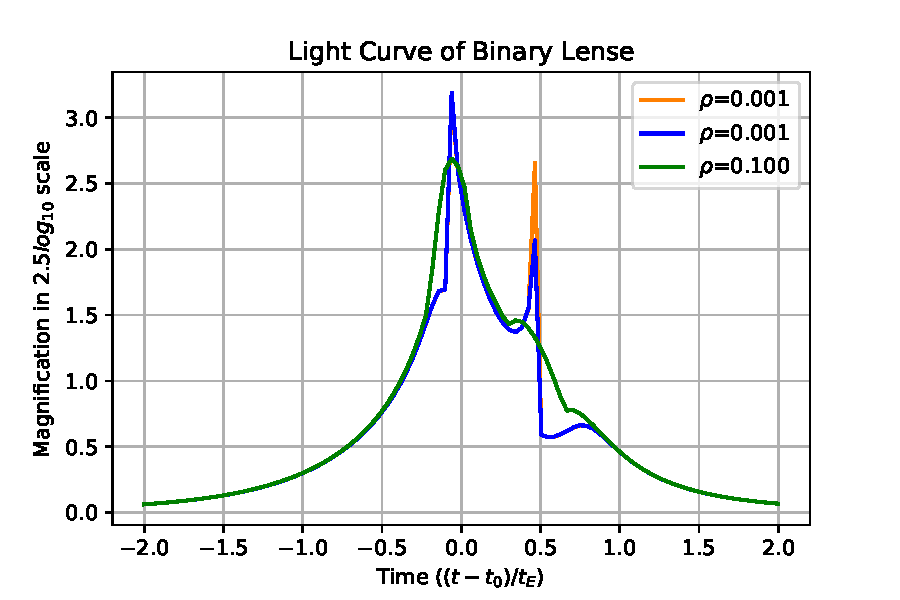
\includegraphics[width=\textwidth]{2_2c_l.png}
  \caption{Light Curve with Different $\rho$}
\end{subfigure}%
\begin{subfigure}{.49\textwidth}
  \centering
  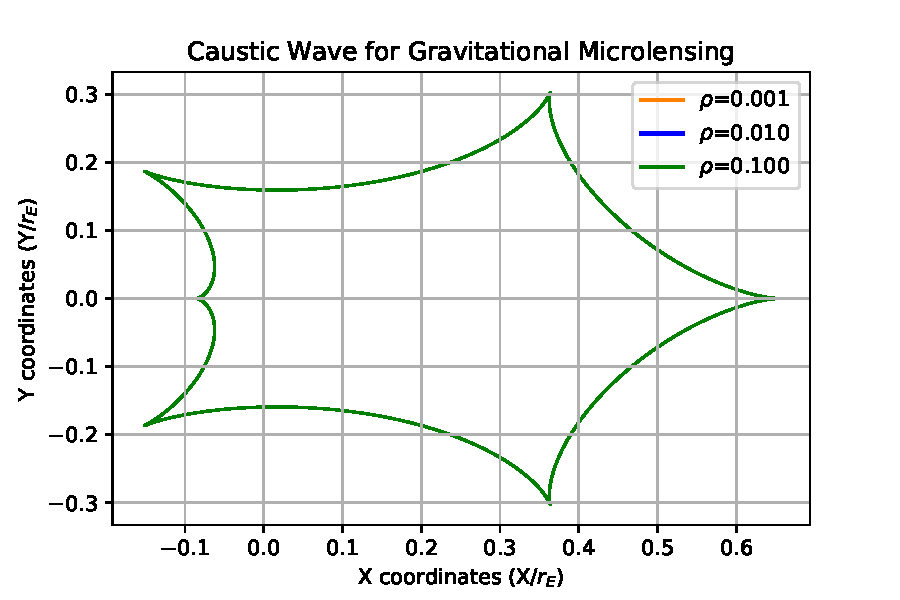
\includegraphics[width=\textwidth]{2_2c_c.png}
  \caption{Caustics Curve with Different $\rho$ }
\end{subfigure}%
\caption{Light Curve and Caustics Wave for Static Binary Lens}
\label{fig 3}
\end{figure}

\bigskip
\bigskip
\bigskip
\bigskip
\bigskip
\subsection{Orbital Motion and Parallax}

In part a, the period ($T$) of the binary orbital motion can be found as with follow equation by Kepler's third law, where $a$ is the semi-major axis, which $a=sr_E$ in this binary lens system \cite{Carroll2007_2}.
\begin{equation}
   T = 2\pi\sqrt{\frac{a^3}{G (M_1 + M_2)}}
\end{equation}
In this case, $M_1=10~M_\odot$, $M_2=1~M_\odot$, $s=1.2$, and $r_{\rm E}=10$ AU. The gravitation constant is $G=39.478 AU^{-3}yr^{-2}M_\odot^{-1}$. y substituting above quantities into equation 6, we can get the orbital period as 12.53 yr.\par
\bigskip
In part b, we assubig the orbit in face-on, therefore the rotating on the sky has fixed separations $s$ that $\frac{ds}{dt}=0$. The parameter that is changing due to the orbital motion of the binary system is the binary axis angle $\alpha$, which the change of $\frac{d\alpha}{dt}$ equals to the angular velocity of the orbital motion $\frac{360}{T}=28.72 deg/yr$. The initial value of binary axis angle $\alpha_0$ is zero. The other parameters are $t_{\rm E}=100$ days, $u_0=0.1$ and $\rho=10^{-3}$. \par
After setting the above parameters in a model using \texttt{MulensModel.binarylens} module, the light curve of the binary lens with orbital motion is determined \texttt{VBBL} method. Similarly, by setting $\frac{d\alpha}{dt}=0$ in the model, the light curve for the static binary lens can be found. By setting $(\pi_{\rm E,N},\,\pi_{\rm E,E})=(0.2,\,0)$ in the static model, the light curve for the static binary lens with parallax can be found. The graph is shown in Figure 4.\par
\begin{figure}[h]
\centering
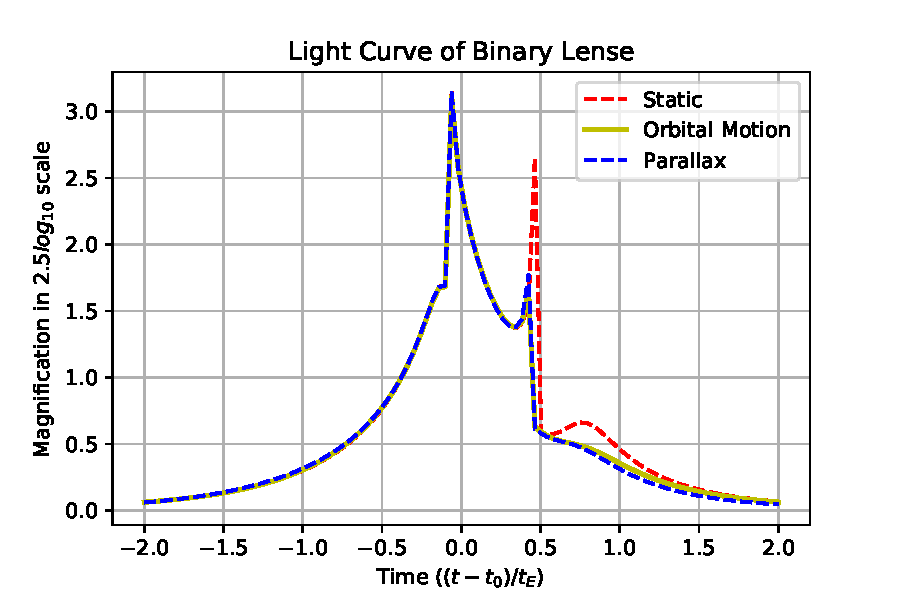
\includegraphics[width=.55\textwidth]{2_3b.png}
\caption{Light Curve of Binary Lens Systems}
\label{fig 4}
\end{figure}
In the graph, the light curve of the system with orbital motion and the system with parallax has very similar light curve. In this case, the light curve is caused by the orbital motion, but if we misunderstand it as the result of the parallax, the mass of the system determined with these two cases can be really different.\par
Let assume the distance from the observer to the lens $D_L$ be 4 kpc, then the parallax $\pi_E$ for orbital motion in this case is:$$\pi_E=\pi/\theta_E=\frac{AU}{4kpc}\frac{D_L}{r_E}=0.1$$
From section 1.4, we know that parallax is proportional to $M_L^{-1/2}$, and $\pi_{E(para)}/\pi_{E(orb)}=2$, therefore $M_{orb}=4M_{para}$. If we consider the light curve due to the parallax instead of orbital motion, the mass we found is four times smaller than the real mass. In this case, the lens object can be a stellar mass blackhole, but the mass we calculated with the parallax is a white dwarf.\par
\bigskip
In part c, once the parameters for the orbital motion, static binary system and the parallax is set in different module with \texttt{MulensModel.Binarylens}. The trajectory of source is determined with the \texttt{MulensModel.trajectory} module and the caustics curve of the static system is found with \texttt{MulensModel.caustics} module. The graph for the trajectory of the three systems and static caustics curve is shown in Figure 5. \par
\begin{figure}[h]
\centering
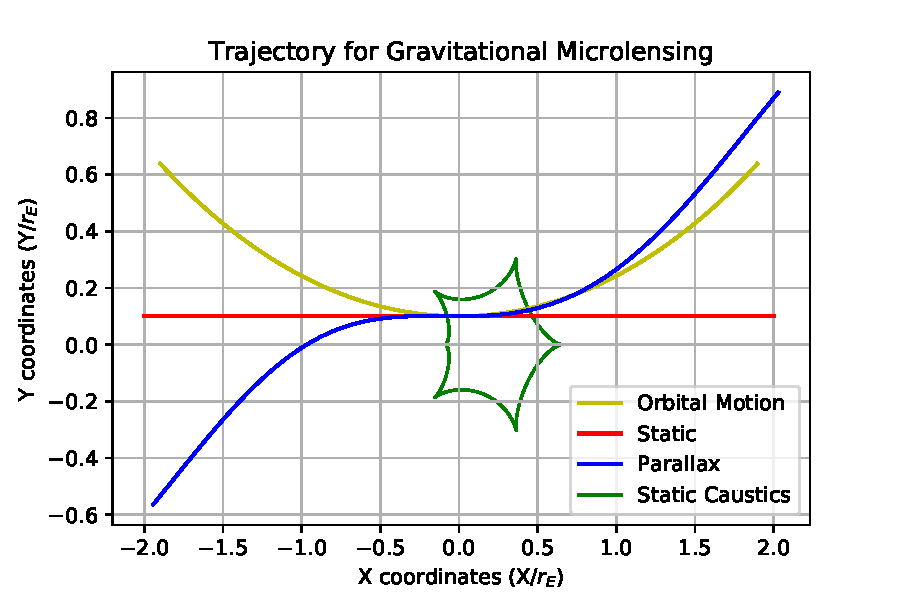
\includegraphics[width=.55\textwidth]{2_3c.png}
\caption{Trajectory and Caustics Curve of Binary Lens Systems}
\label{fig 5}
\end{figure}

From the graph, we can see there is a portion of the trajectory for the orbital motion and parallax system that is the same. The code for 2.3b and 2.3c is in the file microlensing-4.py.
\clearpage
\bibliographystyle{plain}
\bibliography{references}
\end{document}



